\documentclass[12pt]{article}
\usepackage[margin=1.27cm]{geometry}
\usepackage{setspace}
\usepackage{fontspec}
% \usepackage[T1]{fontenc}
% \usepackage[utf8]{inputenc}
\usepackage{amsmath,txfonts,amssymb,nicefrac,mathtools,pifont} %for math
\usepackage{array,tabularx,multirow,fmtcount} %for tables
\usepackage{tikz, pgfplots} %for diagram
\usepackage{multicol} %for multiple column
\usepackage{enumerate,enumitem,adjustbox} %for ordered list
\usepackage{graphicx,subcaption,wrapfig,tcolorbox} %for figure
\usepackage{xparse} %for commands & environments
\usepackage{lipsum} %miscellaneous
\usepackage{colortbl,xcolor,soul} %for default table & border

% #ANCHOR Font settings
\setmainfont{Oxygen}
\newfontfamily\banglafont[Script=Bengali]{Baloo Da 2}
\newfontfamily{\lstsansserif}{IBM Plex Mono}
\renewcommand{\normalsize}{\fontsize{11.5pt}{13pt}\selectfont}


\setlength{\arrayrulewidth}{0.35 pt}
\definecolor{border}{HTML}{A1A1AA}
\arrayrulecolor{border}


% #ANCHOR Document settings
\linespread{1.45}
\setlength\parindent{0pt}
\setlength\parskip{16pt}
\setlist[enumerate]{noitemsep}
\usetikzlibrary{shapes.geometric,decorations.pathreplacing,trees,arrows,positioning,shapes,fit,calc,decorations.markings, decorations.text}
\tikzset{every node/.append style={font=\footnotesize}}
\usepgfplotslibrary{fillbetween}
\pgfdeclarelayer{background}
\pgfsetlayers{background,main}
\pgfplotsset{compat=1.18}
\columnseprule=1pt
\everymath{\displaystyle}
% #ANCHOR Hypernation
\tolerance=1
\emergencystretch=\maxdimen
\hyphenpenalty=10000
\hbadness=10000
\newlength{\colWidth}



% #ANCHOR Colors
\definecolor{azure(colorwheel)}{rgb}{0.0, 0.5, 1.0}
\definecolor{carminepink}{rgb}{0.92, 0.3, 0.26}
\definecolor{orange}{rgb}{0.9, 0.55, 0.22}
\definecolor{violet}{rgb}{0.60, 0.45, 1}
% Syantax Highlighting Colors
\definecolor{keyword}{HTML}{D73A4A}
\definecolor{number}{HTML}{015CC5}
\definecolor{comment}{HTML}{6A737D}
\definecolor{string}{HTML}{1D825E}
\definecolor{function}{HTML}{743FD1}
\definecolor{orange}{HTML}{CF7842}
\definecolor{codeblack}{HTML}{24292F}
\definecolor{divider}{HTML}{A1A1AA}
\definecolor{border}{HTML}{D1D1D1}


% #ANCHOR Ordered & Unordered List
\setlist[itemize,1]{left=0cm, label={\textbullet}}
\setlist[itemize,2,3,4,5,6,7,8,9,10]{left=0.6cm, label={\textbullet}}
\setlist[enumerate,1]{left=0cm}
\setlist[enumerate,2,3,4,5,6,7,8,9,10]{left=0.6cm}
\setul{0.5ex}{0.125ex}



% #ANCHOR Colored Box
\let\oldul\ul
\renewcommand{\ul}[2][keyword]{\text{\setulcolor{#1}\oldul{#2}}}
\newcommand{\redbox}[1]{%
{\color{red}\fbox{\color{black}#1}}
}
\newcommand{\red}[1]{%
\textcolor{red}{#1}
}
\newcommand{\redeq}[1]{%
\text{\color{red}$#1$}
}
\newcommand{\mred}[1]{%
\textcolor{keyword}{#1}
}
\newcommand{\mredeq}[1]{%
\textcolor{keyword}{$#1$}
}
\newcommand{\blue}[1]{%
% {\color{number}#1\hspace{-0.4ex}}
\textcolor{number}{#1}
}
\newcommand{\blueeq}[1]{%
\text{\color{number}$#1$}
}
\newcommand{\cyanbox}[1]{%
{\color{teal}\fbox{\textcolor{black}{#1}}}
}
\newcommand{\cyan}[1]{%
\textcolor{teal}{#1}
}
\newcommand{\pink}[1]{%
\textcolor{magenta}{#1}
}
\newcommand{\orange}[1]{%
\textcolor{orange}{#1}
}
\newcommand{\violet}[1]{%
{\color{violet}#1}
}
\newcommand{\cyaneq}[1]{%
\text{\color{teal}$#1$}
}
\newcommand{\gray}[1]{%
\textcolor{comment}{#1}
}
\newcommand{\pinkeq}[1]{%
\text{\color{magenta}$#1$}
}
\renewcommand{\columnseprulecolor}{\color{divider}}




% #ANCHOR Tabular commands
\newcolumntype{P}[1]{>{\centering\arraybackslash}p{#1}}
\newcolumntype{M}[1]{>{\centering\arraybackslash}m{#1}}
\newcolumntype{C}{>{\centering\arraybackslash}X}
\newcommand{\rspan}[2]{\multirow{#1}{*}{#2}}
\newcommand{\thc}[1]{%
\multicolumn{1}{|c|}{\textbf{#1}}
}
\newcommand{\thcx}[1]{%
\multicolumn{1}{|C|}{\textbf{#1}}
}
\newcommand{\thl}[1]{%
\multicolumn{1}{|l|}{\textbf{#1}}
}
\newcommand{\thr}[1]{%
\multicolumn{1}{|r|}{\textbf{#1}}
}
% Adjusting arraystretch to modify vertical padding
\renewcommand{\arraystretch}{1.25}
% Adjusting tabcolsep to modify horizontal padding
\setlength{\tabcolsep}{10pt}



% #ANCHOR Math commands
\newcommand{\set}[1]{\{$#1$\}}
\newcommand{\tabs}{\ \ \ \ \ \ }
\newcommand{\tab}{\ \ \ }
\newcommand{\cmark}{\ding{51}}%
\newcommand{\xmark}{\ding{55}}%
\newcommand{\boldi}[1]{\boldsymbol{#1}}%
\newcommand{\wspace}{\ \ = \ \ }



% #ANCHOR New commands
\newcommand{\Title}[1]{%
   \begin{center}
      \textbf{\Large{#1}}
   \end{center}
}
\newcommand{\Heading}[1]{%
   \par\vspace{\dimexpr -\baselineskip + 16pt}
   {\fontsize{12pt}{13pt}\selectfont\textbf{#1}}
   \par\vspace{\dimexpr -\baselineskip + 6pt}
}
\newcommand{\BuleHeading}[1]{%
   \par\vspace{\dimexpr -\baselineskip + 16pt}
   {\fontsize{12pt}{13pt}\selectfont\textbf{\textcolor{number}{#1}}}
   \par\vspace{\dimexpr -\baselineskip + 6pt}
}
\newcommand{\CHeading}[1]{%
   \par\vspace{\dimexpr -\baselineskip + 16pt}
   \hspace{\fill}
   {\fontsize{12pt}{13pt}\selectfont\textbf{#1}}
   \hspace{\fill}
   \par\vspace{\dimexpr -\baselineskip + 6pt}
}
\newcommand{\Section}[1]{%
   \par\vspace{\dimexpr -\baselineskip + 16pt}
   \hspace{\fill}
   {\fontsize{13pt}{13pt}\selectfont\textbf{#1}}
   \hspace{\fill}
   \par\vspace{\dimexpr -\baselineskip + 6pt}
}
\newcommand{\seteqno}[1]{%
   \ \cdots \ \cdots \ \cdots \ (#1)
}
\newcommand{\eqor}{%
   \Rightarrow \ \ 
}
\newcommand{\tsub}[1]{%
\textsubscript{#1}\hspace{-0.45ex}
}
\newcommand{\tsup}[1]{%
\textsuperscript{#1}\hspace{-0.45ex}
}
\newcommand{\cbox}[2][cyan]{
\tikz\node[draw=#1,circle,inner sep=2pt,baseline=(a.base)](a){#2};
}
\newcommand{\hrline}{%
\vspace{1ex} {\color{gray}\hrule} \vspace{4ex}
}
\newcommand{\divideX}[1][divider]{{\hspace{1ex}\color{#1}{\vrule}\hspace{1ex}}}
\newcommand{\Reference}[2][Reference]{

\vspace{-0.5\baselineskip}
\begin{center}
   {\fontspec{Merriweather}\textbf{#1:} \textit{#2}} 
\end{center}
}
\newcommand{\bn}[1]{%
   {\banglafont #1}
}

\NewDocumentCommand{\Column}{O{0.49} O{1.5em} m m}{
   \setlength{\colWidth}{\linewidth-#1\linewidth-#2}
   \begin{minipage}[t]{#1\linewidth}
      \noindent
         #3
      \end{minipage}\hspace{\fill}{\color{divider}\vrule width 0.35pt}\hspace{\fill}
      \begin{minipage}[t]{\colWidth}
      \noindent
         #4
   \end{minipage}
}

\usepackage{circuitikz}
\newcommand{\ac}[1]{#1 to[sV, fill=white] #1}

\begin{document}
\Lecture{EEE Final Lecture}

\vspace{4ex}
\Lecture{DC Circuit}
\vspace{-0.75\baselineskip}

\Heading{Circuit analysis: \cyan{Node analysis}}
\begin{enumerate}[itemsep=0ex]
   \item Identify all nodes.
   \item Let ground reference node.
   \item Label non-reference nodes.
   \item Write a KCL equation for each node using Ohm's Law.\\
   (sum the currents leaving the node and set equal to zero)
   \item Solve those equations for voltages.
\end{enumerate}
\hspace{1ex}
\begin{tabular}{l}
   \textbf{Note:} Reference node \bn{এবং} non-reference node \bn{এর মাঝখানে যদি কোন} voltage source \bn{থাকে, তবে সেই} \\voltage source \bn{এর} voltage\bn{-ই হবে} non-reference node \bn{এর} voltage\bn{।}
\end{tabular}

\vspace{1ex}
\Heading{Circuit analysis: \cyan{Mesh analysis}}
\begin{enumerate}[itemsep=0ex]
   \item Identify the meshes/loops.
   \item Assign a current variable to each loop, using a consistent direction.\\(clockwise or counterclockwise)
   \item Write a KVL equations for each loop using Ohm's Law
   \item Solve those equations for loop currents.
   \item Solve for other element currents and voltages you want using Ohm'sLaw.
\end{enumerate}

\hspace{1ex}
\begin{tabular}{l}
   \textbf{Note:} \bn{যদি কোন লুপে একটা মাত্র} current source \bn{থাকে, তবে সেটিই হবে ঐ লুপের} loop current \bn{হবে।} 
\end{tabular}

\pagebreak
\vspace*{-2\baselineskip}
\Heading{Circuit theorem: \cyan{Superposition}}
\begin{enumerate}[itemsep=0ex]
   \item Open current sources and short voltage sources.
   \item Find the output (voltage or current) due to that active source using nodal or mesh analysis.
   \item Repeat step 1 \& 2 for each of the other independent sources.
   \item Find the total contribution by adding algebraically all the contributions due to the independent sources.
\end{enumerate}

\Heading{Circuit theorem: \cyan{Thevenin}}
\begin{enumerate}[itemsep=0ex]
   \item Open Current Sources, Short Voltage Sources and Open Load Resistor.
   \item Calculate the open circuit resistance. This is the Thevenin resistance (R$_{TH}$).
   \item Calculate the open circuit voltage. This is the Thevenin Voltage (V$_{TH}$).
   \item Now, redraw the circuit with measured V$_{TH}$ and R$_{TH}$. This is the equivalent Thevenin circuit.
   \item Now find the total current flowing through load resistor by using the Ohm's Law: $\text{I}_T = \frac{\text{V}_{TH}}{(\text{R}_{TH}+\text{R}_L)}$.
\end{enumerate}

\Heading{Circuit theorem: \cyan{Norton}}
\begin{enumerate}[itemsep=0ex]
   \item Short the load resistor.
   \item Calculate the short circuit current. This is the Norton Current $($I$_{N})$.
   \item Open Current Sources, Short Voltage Sources and Open Load Resistor.
   \item Calculate the open circuit resistance. This is the Norton resistance $($R$_{N})$.
   \item Now, redraw the circuit with measured I$_{N}$ and R$_{N}$. This is the equivalent Norton circuit.
   \item Now find the Load current flowing through load resistor by using Current divider rule.
\end{enumerate}

\hspace{1ex}
\begin{tabular}{l}
\textbf{Tips:} Use Thevenin theorem to calculate V$_{TH}$ and R$_{TH}$. Then $\text{I}_{N} = \frac{\text{V}_{TH}}{\text{R}_{TH}}$
\end{tabular}

 
\pagebreak
\vspace*{-\baselineskip}
\Lecture{AC Circuit}
\vspace{-0.75\baselineskip}
\Heading{Class-1: \cyan{Complex numbers}}
\Reference[Exercise]{14.15-14.26 | Page: 600}

\vspace{3ex}
\begin{minipage}[t]{0.4\textwidth}
   \begin{tabular}{ll|}
      \ Rectangular \ &: \ \large{${a} \pm j{b}$} \\
      \ Trigonometrical \ &: \ \large{${E}(\cos{{\theta}} \pm \sin{{\theta}})$} \\
      \ Exponential \ &: \ \large{${E} \cdot e^{j{\theta}}$} \\
      \ Polar \ &: \ \large{${E} \ \angle \pm {\theta} $} \\
   \end{tabular}
\end{minipage}
\hfill
\begin{minipage}[t]{0.56\textwidth}
   \vspace{-2\baselineskip}
   \begin{tabular}{ll}
      \large{$E=\sqrt{a^2+b^2}$} & \large{$a = E \cos{\theta}$}\\[0.8ex]
      \large{$\theta = \tan^{-1}{\frac{b}{a}}$} & \large{$b = E \sin{\theta}$}\\[0.8ex]
      $\bullet$ Use Rectangular form for &: \ $+\ , -$ \\
      $\bullet$ Use Polar form for &: \ $\times \ , \div$
   \end{tabular}
\end{minipage}



\vspace{5ex}
\Heading{Class-2: \cyan{Sinusoidal Expression}}
\Reference[Exercise]{14.2-14.7 | Page: 584}

\vspace{2ex}
\begin{minipage}[t]{0.33\textwidth}
   \begin{center}
   \begin{circuitikz}
      \draw
      (0,0) -- (5,0) -- (5,2.5) -- (3.1,2.5) (1.9,2.5) -- (0,2.5) -- (0,0)
      \ac{(2.5, 0)}
      (2, 2.5) to[R, fill=white] (3, 2.5);
  \end{circuitikz}\\
  Pure Resistive
  $$v=V_m \sin{\omega t}$$\\[-2.5\baselineskip]
  $$i = I_m \sin{\omega t}$$\\[-2\baselineskip]
  $$I_m = \frac{V_m}{R}$$
  \end{center}
\end{minipage}
\begin{minipage}[t]{0.33\textwidth}
   \begin{center}
   \begin{circuitikz}
      \draw
      (0,0) -- (5,0) -- (5,2.5) -- (3.1,2.5) (1.9,2.5) -- (0,2.5) -- (0,0)
      \ac{(2.5, 0)}
      (1.8, 2.5) to[L, fill=white] (3.2, 2.5);
  \end{circuitikz}\\
  Pure Inductive
  $$v=V_m \sin{\omega t}$$\\[-2.5\baselineskip]
  $$i = I_m \sin{(\omega t - 90^{\circ})}$$\\[-2\baselineskip]
  $$I_m = \frac{V_m}{X_L} = \frac{V_m}{\omega L}$$
  \end{center}
\end{minipage}
\begin{minipage}[t]{0.33\textwidth}
   \begin{center}
   \begin{circuitikz}
      \draw
      (0,0) -- (5,0) -- (5,2.5) -- (3.1,2.5) (1.9,2.5) -- (0,2.5) -- (0,0)
      \ac{(2.5, 0)}
      (1.8, 2.5) to[C, fill=white] (3.2, 2.5);
  \end{circuitikz}\\
  Pure Capacitive
  $$v=V_m \sin{\omega t}$$\\[-2.5\baselineskip]
  $$i = I_m \sin{(\omega t + 90^{\circ})}$$\\[-2\baselineskip]
  $$I_m = \frac{V_m}{X_C} = \frac{V_m}{\frac{1}{\omega C}}$$
  \end{center}
\end{minipage}

\vspace{2ex}
\begin{minipage}[t]{0.33\textwidth}
   \includegraphics[width=5.6cm]{figures/Pure Resistive.JPG}
\end{minipage}
\begin{minipage}[t]{0.33\textwidth}
   \includegraphics[width=5.6cm]{figures/Pure Inductive.JPG}
\end{minipage}
\begin{minipage}[t]{0.33\textwidth}
   \includegraphics[width=5.6cm]{figures/Pure Capacitive.JPG}
\end{minipage}

\Heading{Class-3: \cyan{Impedance}}

\vspace{-0.5\baselineskip}
\Reference[Exercise]{16.1, 16.2, 16.3}


\textbf{Impedance $(z)$:} \ The ratio of the phasor voltage $(V)$ to the phasor current $(I)$ in ohms.

\begin{itemize}
   \item In pure resistive circuit, volatge $(v)$ and current $(i)$ stay in phase.\\[-5ex]
   \item In pure inductive circuit, voltage $(v)$ leads the current $(i)$ by 90°.\\[-5ex]
   \item In pure capacitive circuit, current $(i)$ leads the voltage $(v)$ by 90°.
\end{itemize}

\vspace{1ex}
\begin{center}
   \begin{tabular}{|r|l|l|}
      \hline
       & \textbf{Impedance} in & \textbf{Impedance} in\\[-1ex]
      \textbf{Element}&Rectangular form&Polar form\\\hline
     (Resistor) R & $\mathrm{Z}_R \ = \ \mathrm{R}$ & \ $\mathrm{Z}_R \ \angle 0^\circ$\\\hline
     (Inductor) L & $\mathrm{Z}_L \ = \ \mathrm{j\ X_L} \ = \ \mathrm{j \omega L}$ & \ $\mathrm{Z}_L \ \angle 90^\circ$\\\hline
     (Capacitor) C & $\mathrm{Z}_C \ = \ -\mathrm{j\ X_C} \ = \ -\mathrm{j} \frac{1}{\mathrm{\omega C}}$ & \ $\mathrm{Z}_C \ \angle -90^\circ$\\[0.8ex]\hline
   \end{tabular}
\end{center}


\vspace{5ex}
\Heading{Class-4: \cyan{Power Factor}}

\vspace{-0.5\baselineskip}
% \Reference[Exercise]{14.2-14.7 | Page: 584}
P.f is a measure of how effectively electrical equipment converts electric power into useful power.
\vspace{3ex}

\begin{minipage}[t]{0.56\linewidth}
   \begin{enumerate}
      \item Pf is the ratio of active power to the total power.
      \vspace{-0.5\baselineskip}
      $$P.f = \frac{\mathrm{Active \ power}}{\mathrm{Total \ power}} = \frac{P}{S} = \frac{P}{P+Q}$$
      
      \vspace{-0.75\baselineskip}
      \item The cosine angle between the current and the voltage is called pf.
      \vspace{-0.75\baselineskip}
      \begin{align*}
         \mathrm{Pf} & = \cos{\theta}\\
         \mathrm{P} & = \mathrm{VI} \cos{\theta} \ \ (watt)\\
         \mathrm{Q} & = \mathrm{VI} \sin{\theta} \ \ (VAR)\\
      \end{align*}
   \end{enumerate}
\end{minipage}
\hspace{5ex}
\begin{minipage}[t]{0.3\linewidth}
   \vspace{-0.5\baselineskip}
   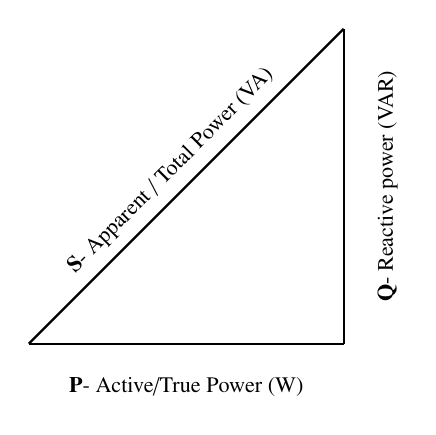
\begin{tikzpicture}
      \draw [thick] (0,0) -- (4,4)
      node[midway, sloped, above]{\textbf{S}- Apparent / Total Power (VA)};
      \draw [thick] (0,0) -- (4,0)
      node[midway, sloped, below=8pt]{\textbf{P}- Active/True Power (W)};
      \draw [thick] (4,0) -- (4,4)
      node[midway, sloped, below=8pt]{\textbf{Q}- Reactive power (VAR)};
   \end{tikzpicture}
\end{minipage}






\pagebreak
\vspace*{-\baselineskip}
\Lecture{Magnetic Circuit}
\vspace{-0.75\baselineskip}
\Heading{Class-1: \cyan{Formulas}}



\begin{minipage}[t]{0.45\linewidth}
   \noindent
   \Topic{Flux density:}
   \begin{tabular}{l|l}
      \rspan{2}{$B = \mathrm{\frac{\Phi}{A}}$}
      & $\mathrm{\Phi}$ = Flux \ ($\mathrm{Wb}$) \\
      & $\mathrm{A}$ = Area \ ($\mathrm{m^2}$)
   \end{tabular}

   \vspace{3ex}
   \Topic{Permeability:}
   \begin{tabular}{l|l}
      \rspan{2}{{$\mu = {\frac{B}{H}}$}}
      & ${B}$ = flux density \ ($\mathrm{T}$)\\
      & ${H}$ = magnetizing force \ ($\mathrm{At/m}$)\\
   \end{tabular}

   \vspace{3ex}
   \Topic{Realtive Permeability:}
   \begin{tabular}{l|l}
      {$\mu_r = \frac{\mu}{\mu_o}$}
      & $\mu_o = 4\pi \times 10^7$ \ \ ($\mathrm{Wb/A.m}$)
   \end{tabular}
\end{minipage}\vline\hspace{1ex}
\begin{minipage}[t]{0.45\linewidth}
   \noindent
   $$NI = Hl$$
   \begin{tabular}{ll}
      Where,
      & ${H}$ = magnetizing force \ ($\mathrm{At/m}$) \\
      & ${B}$ = flux density \ ($\mathrm{T}$)\\
      & ${I}$ = current \ ($\mathrm{A}$)\\
      & ${l}$ = length \ ($\mathrm{m}$) \\
   \end{tabular}

   \vspace{3ex}
   $\star$ 1 mitre = 39.37 inch\\
   $\star$ l = total length \\[2ex]
   E.g: $l_{ab} = l_{cd} = 0.5 \ \mathrm{in}$ \ \ and \ \ $l_{bc}=4 \ \mathrm{in}$\\
   $\therefore l = 0.5 + 4 + 0.5 = 5 \ \mathrm{in} =  \ \frac{5}{39.37} \ \mathrm{m}$

\end{minipage}






\end{document}
